\FILENAME

\chapter{Frequently Asked Questions}\label{frequently-asked-questions}

\section{General}\label{general}

\subsection{What is Chameleon?}\label{what-is-chameleon}

Chameleon is an experimental testbed for Computer Science funded by the
NSF FutureCloud program. Chameleon is built over two sites, University
of Chicago and TACC, offering a total of over 550 nodes and 5 PB of
space in twelve
\href{https://www.chameleoncloud.org/about/hardware-description/}{Standard
Cloud Unit (SCU) racks}. To effectively support Computer Science
experiments Chameleon offers bare metal reconfigurability on most of the
hardware. To provide easy access to educational users, three SCUs at
TACC (a quarter of the testbed) are configured with OpenStack KVM. You
can read more about
Chameleon~\href{https://www.chameleoncloud.org/about/chameleon/}{here}.

\subsection{What does CHI mean?}\label{what-does-chi-mean}

CHI stands for Chameleon Infrastructure, and refers to the technology
powering our bare-metal clouds: a combination of software components
from OpenStack, Grid'5000, and our own~developments.

\subsection{Who can use Chameleon?}\label{who-can-use-chameleon}

Chameleon is broadly available to members of the US Computer Science
research community and its international collaborators working in the
open community on cloud research. ~By emphasizing ``open'' we mean that
the expectation is that any research performed on Chameleon will result
in publication in a broadly available journal or conference.~

\subsection{What are the best practices for Chameleon
usage?}\label{what-are-the-best-practices-for-chameleon-usage}

In order to promote fairness to all users, we have~the following set of
Best Practices for using Chameleon~bare metal partitions:

\begin{itemize}
\tightlist
\item
  ~Think Small for Development: If you are just developing or
  prototyping a system, and not yet running experiments at scale, use
  only as many nodes as you actually need (e.g., many projects can be
  developed and tested on 3-4 nodes), and try to take short reservations
  (e.g., for a work day or two when you actually develop). Always
  release the reservation if you will not use the testbed for an
  extended period of time (e.g., when you leave for the weekend or
  holidays).~
\item
  Automation is your Friend: You can always snapshot your work/images
  between sessions using the
  \href{https://www.chameleoncloud.org/docs/user-guides/ironic/\#snapshotting_an_instance}{snapshotting
  instructions}~to simplify the redeployment of your environment during
  the next work session. You can also use scripting and environment
  customization to make it easier to redeploy images. An additional
  benefit of automation is that it makes it easier for you to reproduce
  your work and eventually~share it~with colleagues within your lab and
  other collaborators.
\item
  Think Big for Experimentation: Once you are ready to experiment you
  will want to test your experimental setup on increasingly larger
  scales. This is possible by taking an advance reservation for many
  resources for a relatively short time. The more resources you need,
  the more likely it is that you will need to run experiments at a less
  attractive time (e.g., during the weekend) --- here's where automation
  will also help. In justified cases, we will support reserving even the
  whole bare metal testbed.
\end{itemize}

\subsection{Are there any limitations on Chameleon
usage?}\label{are-there-any-limitations-on-chameleon-usage}

We have two types of limitations, introduced to promote fair resource
usage to all:~

\begin{itemize}
\tightlist
\item
  Allocation:~Chameleon projects are limited to a per-project allocation
  currently set to~20,000 service units for 6 months. Allocations can be
  renewed or extended---see the
  \href{index.html\#toc-project-and-allocation-management}{Project and
  Allocation Management} section for more details on Chameleon
  allocations.
\item
  Lease: To ensure fairness to all users, resource reservations (leases)
  are limited to a duration of 7 days. However, an active lease within
  48 hours of its end time can be prolonged by up to 7 days from the
  moment of request if resources are available. To prolong a lease,
  click on the ``Update Lease'' button in the Reservations panel of the
  CHI OpenStack dashboard, and enter the additional duration requested
  in the ``Prolong for'' box including the unit suffix, e.g. ``5d'' for
  5 days or ``30m'' for 30 minutes. If there is an advance reservation
  blocking your lease prolongation that could potentially be moved, you
  can interact through the users mailing list to coordinate with others
  users.~Additionally, if you know from the start that your lease will
  require longer than a week and can justify it, you can
  \href{https://www.chameleoncloud.org/user/help/ticket/new/}{contact
  Chameleon staff via the ticketing system} to request a one-time
  exception to create a longer lease.
\end{itemize}

\subsection{How should I acknowledge Chameleon in my
publications?}\label{how-should-i-acknowledge-chameleon-in-my-publications}

An acknowledgement of support from the Chameleon project and the
National Science Foundation should appear in any publication of
material, whether copyrighted or not, that describes work which
benefited from access to Chameleon cyberinfrastructure resources. The
suggested acknowledgement is as follows: ``Results presented in this
paper were obtained using the Chameleon testbed supported by the
National Science Foundation''.

\subsection{What infrastructures is Chameleon federated
with?}\label{what-infrastructures-is-chameleon-federated-with}

Chameleon supports identity federation with GENI designed to give GENI
users immediate access to Chameleon without having to create a Chameleon
account or project. GENI users can log in with their GENI credentials
and charge their usage the GENI Federation Project created to provide
startup cycles to researchers evaluating Chameleon. To obtain a larger
allocation focused on their research needs, GENI users can then go on to
create individual Chameleon projects. Chameleon users can also log in to
the GENI Experimenter Portal using their Chameleon credentials. When
selecting the organization with whom to log in to GENI, search for
``Chameleon Cloud'' in the list of Identity Providers. You will be
redirected to the Chameleon Auth Service to log in and then back to the
GENI Experimenter Portal upon successful login.

\section{Project and Allocation
Management}\label{project-and-allocation-management}

\subsection{How do I apply for a Chameleon
project?}\label{how-do-i-apply-for-a-chameleon-project}

Project applications may be filled out
\href{https://www.chameleoncloud.org/user/projects/new/}{here}. If you
want to apply for a project you have to be
\href{https://www.chameleoncloud.org/docs/getting-started/pi-eligibility/}{PI
eligible}; if you fulfill the PI eligibility criteria but did not
request PI eligibility when you applied for a Chameleon account you can
request it by modifying options in your profile. An application for a
project has to include a description of the research or education
project to be performed using the testbed and the type of resources
needed (see below). Each Chameleon project is awarded an allocation of
service units for a specific amount of time.~Users can expect a project
decision within one~business day.

\subsection{Who is eligible to be Chameleon PI and how do I make sure
that my PI status is reflected in my
profile?}\label{who-is-eligible-to-be-chameleon-pi-and-how-do-i-make-sure-that-my-pi-status-is-reflected-in-my-profile}

Chameleon PIs carry significant responsibility for the users on their
projects; we therefore limit PI eligibility to individual from the
following groups:

\begin{itemize}
\tightlist
\item
  Academic institutions: This eligibility criterion coves research
  scientists or faculty members in those institutions
\item
  Federal agencies such as national labs, R\&D centers, and institutes:
  Research staff employed by federal agencies or non-NSF Federally
  Funded R\&D Centers (FFRDCs) are eligible to apply for an allocation.
\item
  Independent museums, observatories, libraries, research laboratories,
  professional societies and similar organizations in the United States
  that are directly associated with educational or research activities
  are eligible.
\item
  International research institutions: to promote intellectual exchange
  and federation with institutions abroad we support a limited number of
  international PIs with ongoing, active collaborations with scientists
  in the US.~
\item
  NSF Graduate Student Fellows: While in most cases, a graduate student
  is ineligible to be PI of an allocation request, an exception is made
  for NSF Graduate Student Fellows. Recipients of these NSF awards can
  submit requests for Startup allocations as long as they include
  supporting documentation (grant number or an award letter) as part of
  the request submission.
\item
  State educational offices or organizations and local school districts
  may submit allocation requests intended to broaden the impact,
  accelerate the pace, and increase the effectiveness of improvements in
  science, mathematics, and engineering education in both K-12 and
  post-secondary levels. A teacher or educator at an accredited public
  or private K-12 school is eligible to apply for an allocation as PI.
\end{itemize}

We do occasionally provide case-by-case exceptions to this guideline in
well-justified cases.~

If are eligible to be PI, in order to apply for a project ~you need to
make sure that your Chameleon profile reflects your status. You can do
so on the~\href{https://www.chameleoncloud.org/user/profile/edit}{Edit
Account Profile page}. Simply check the ``Request PI Eligibility''
checkbox and save you Account Profile.

\subsection{My PI/Professor/Colleague already has a Chameleon Project.
How do I get added as a user on the
project?}\label{my-piprofessorcolleague-already-has-a-chameleon-project.-how-do-i-get-added-as-a-user-on-the-project}

You will need to contact the project PI and request that they add you as
a user. Provide the PI with your Chameleon username. The project PI
should visit
the~\href{https://www.chameleoncloud.org/user/projects}{Chameleon
Project Management page}. From the list of projects, locate the project
to which the user is to be added and click

View Project

. Near the bottom of the page, under the heading~\emph{Project Users},
is a form where the PI can enter the Chameleon username of the user to
add. Clicking

Add user

~will add the user to the project.

\subsection{What are the units of an allocation, and how am I
charged?}\label{what-are-the-units-of-an-allocation-and-how-am-i-charged}

Chameleon allocations can consist of several components of the system.
Users can request allocation of individual compute nodes, storage
servers, or complete Scalable Compute Units (SCUs) which contain compute
servers, storage nodes, and an open flow switch.

Compute servers are allocated in Service Units (SUs), which equates to
one hour of wall clock time on a single server (for virtual machines, an
SU is 24 cores with up to 128GB of RAM). Note this unit differs from
traditional HPC or cloud service units that are charged in core-hours; a
Chameleon SU is a full server, as the type of experiments and
performance measurements users may wish to do may be contaminated by
sharing nodes.

Storage servers are also charged in SUs, at 2x the rate of compute
servers (i.e., 1 hour allocation of 1 storage server == 2 SUs). SCUs are
charged at the rate of 50 SUs per wall clock hour (42 compute servers, 4
storage nodes, plus one OpenFlow switch).

An allocation may make use of multiple SCUs, up to the size of the full
testbed.

For example, a user wishing to provision a 10 node cluster +1 storage
server for a 1 week experiment should budget
\texttt{{[}(10\ +\ 2)\ SUs\ per\ hour{]}\ *\ {[}7\ days\ *\ 24\ hours/day{]}\ =\ 2,016\ SUs}
for that experiment.

SUs are charged the same regardless of use case. Hence, whether asking
for bare metal access, virtual machine access, or use of default images,
the charge is the same --- you are charged for the fraction of the
resource your experiment occupies, regardless of the type of the
experiment.

The basic principle for charging service units for Chameleon resources
is to evaluate the amount of time a fraction of the resource is
unavailable to other users. If a reservation is made through the portal
for a particular date/time in the future, the user will be charged for
this time regardless of whether the reservation is actually used, as the
Chameleon scheduling system will have to drain the appropriate part of
the system to satisfy the reservation, even if the nodes requested are
not actually used. A reservation request may be cancelled in which case
no charges will apply.

\subsection{What are the project allocation sizes and
limits?}\label{what-are-the-project-allocation-sizes-and-limits}

In the initial phase Chameleon is operating on a ``soft allocation
model'' where each project, if approved, will receive a startup
allocation of 20,000 SUs for six months that can be both recharged
(i.e., more SUs can be added) and renewed (i.e., the duration can be
extended) via submitting a renew/recharge request. This startup
allocation value has been designed to respond to both PI needs (i.e.,
cover an amount of experimentation needed to obtain a significant
result) and balance fairness to other users (it represents roughly 1\%
of testbed six months' capacity). Requests for these startup projects
will receive a fast track internal review (i.e., users can expect them
to be approved within a few days).

A PI can apply for multiple projects/allocations; however, the number of
held allocations will be taken into account during review.

As our understanding of user need grows we expect the Chameleon
allocation model to evolve towards closer reflection of those needs in
the form of more differentiated allocations that will allow us to give
larger allocations to users for longer time.

\subsection{What is the format of an allocation
proposal?}\label{what-is-the-format-of-an-allocation-proposal}

A Chameleon Allocation request consists of the following components:

\begin{itemize}
\tightlist
\item
  Project Title
\item
  Project abstract describing the proposed experiments including the
  type of resources needed; this part is required and may be published
  on Chameleon website (\textasciitilde{}200 words)
\item
  Supplemental details; this is an optional extension of the project
  abstract, potentially including details that the PI does not wish to
  publish such as e.g., sources of funding that support the proposed
  research (500 words maximum)
\end{itemize}

\subsection{According to what criteria are project proposals
reviewed?}\label{according-to-what-criteria-are-project-proposals-reviewed}

Requests for projects and allocations are currently reviewed for merit
by project operators with a future move towards review by independent
review board composed of Chameleon Science Advisory Board members. The
following criteria are used:

\begin{itemize}
\tightlist
\item
  PI eligibility
\item
  Relevance of the proposed experiment to cloud computing research;
  scientific merit and significance of the proposed experiments
\item
  Demonstrated need for Chameleon resources, methodology appropriate to
  the use of the Chameleon resource, justification of the requested
  allocation
\item
  Success of prior or other existing allocations (for renewals) in terms
  of published research results and new funding.
\item
  Technical feasibility (i.e, can the project succeed in the Chameleon
  environment?)
\item
  Any funded support for the project (optional, but we want to make
  certain that we give allocations to NSF CISE-supported cloud computing
  research!).
\end{itemize}

\section{Account Management
Troubleshooting}\label{account-management-troubleshooting}

\subsection{When I attempt to create an account it says my email is
already registered; why does it
happen?}\label{when-i-attempt-to-create-an-account-it-says-my-email-is-already-registered-why-does-it-happen}

Chameleon relies on TACC's Identity Service for account management. If
you already have a TACC account, possibly
through~\href{http://www.xsede.org}{XSEDE}~or directly through TACC,
then you should use that account to log in to Chameleon. If you don't
know your TACC password, you
can~\href{https://www.chameleoncloud.org/password-reset}{reset your
password}. After resetting your password you should be able to log in to
Chameleon.

\subsection{I cannot log into the portal after creating an account, what
should I
do?}\label{i-cannot-log-into-the-portal-after-creating-an-account-what-should-i-do}

Please make sure that you have successfully confirmed your email
address. Check your junk folder as the confirmation email might have
been marked as spam.\textbf{~}Double- check that you are using the
password that you provided during the registration. If you are unsure of
the password you used, you
can~\href{https://www.chameleoncloud.org/user/password-reset/}{reset
it}. If you still cannot log in,
please~\href{https://www.chameleoncloud.org/user/help/ticket/new/guest/}{open
a ticket}.

\subsection{I have an account, but when I try to log in to
OpenStack/Experiment it says my username/password is unknown,
why?}\label{i-have-an-account-but-when-i-try-to-log-in-to-openstackexperiment-it-says-my-usernamepassword-is-unknown-why}

You must be a member of~an active project to access the
OpenStack/Experiment interface. If you are PI Eligible, you can request
a new project on
the~\href{https://www.chameleoncloud.org/user/projects}{Chameleon
Project Management page}. If you are not PI Eligible, you will need to
be added to an existing project by the project PI. You can check that a
project has an active Chameleon allocation by clicking on
the~\textbf{View Project}~button. If you are part of a project but the
allocation is~\emph{Pending}, it means your project is under review. If
you still cannot log in,
please~\href{https://www.chameleoncloud.org/user/help/}{open a ticket
with our help desk}.

\section{Appliances}\label{appliances}

\subsection{What is an appliance?}\label{what-is-an-appliance}

An appliance is an application packaged together with the environment
that this application requires. For example, an appliance can consists
of the operating system, libraries and tools used by the application,
configuration features such as environment variable settings, and the
installation of the application itself. Examples of appliances might
include a KVM virtual machine image, a Docker image, or a bare metal
image. Chameleon appliance refers to bare metal images that can be
deployed on the Chameleon testbed. Since an appliance captures the
experimental environment exactly, it is a key element of
reproducibility; publishing an appliance used to obtain experimental
results will go a long way to allowing others to reproduce and build on
your research easily.

To deploy distributed applications on several~Chameleon instances,
complex appliances combine an~image and a~template describing how the
cluster should be configured and contextualized. You can read more about
them in the
\href{https://www.chameleoncloud.org/docs/complex-appliances/}{Complex
Appliances documentation}.

\subsection{What is the Chameleon Appliance
Catalog?}\label{what-is-the-chameleon-appliance-catalog}

\href{https://www.chameleoncloud.org/appliances/}{The Chameleon
Appliance Catalog}~is a repository that allows users to discover,
publish, and share appliances. The appliance catalog contains useful
images of both bare metal and virtual machine appliances supported by
the Chameleon team as well appliances contributed by users.

\subsection{How do I publish an appliance in the Chameleon Appliance
Catalog?}\label{how-do-i-publish-an-appliance-in-the-chameleon-appliance-catalog}

The new Appliance Catalog allows you to easily publish and share your
own appliances so that others can discover them and use them either to
reproduce the research of others or as a basis for their own research.
~Before creating your own appliance it is advisable to review other
appliances on
the~\href{https://www.chameleoncloud.org/appliances/}{Chameleon
Appliance Catalog}~in order to get an idea of the categories you will
want to contribute and what others have done.~

Once you are ready to proceed, an appliance can be contributed to
Chameleon in the following steps:

\begin{enumerate}
\tightlist
\item
  Create the appliance itself. You may want to test it as well as give
  some thought to what support you are willing to provide for the
  appliance (e.g., if your group developed and supports a software
  package, the appliance may be just a new way of packaging the software
  and making it available, in which case your standard support channels
  may be appropriate for the appliance as well).
\item
  Upload the appliance to the Chameleon Image Repository (Glance) and
  make the image public. In order to enter the appliance into the
  Catalog you will be asked to provide the Glance ID for the image.
  These IDs are per-cloud, so that there are three options right now:
  bare metal/CHI at University of Chicago, bare metal/CHI at TACC, and
  OpenStack/KVM at TACC. You will need to provide at least one
  appliance, but may want to provide all three.
\item
  Go to
  the~\href{https://www.chameleoncloud.org/appliances/create/}{Appliance
  Catalog Create Appliance web form}, fill out, and submit the form. Be
  prepared to provide the following information: a descriptive name
  (this sometimes requires some thought!), author and support contact,
  version, and an informative description. The description is a very
  important part of the appliance record; others will use it to evaluate
  if the appliance contains tools they need for their research so it
  makes sense to prepare it carefully. To make your description
  effective you may want to think of the following questions: what does
  the appliance contain? what are the specific packages and their
  versions? what is it useful for? where can it be deployed and/or what
  restrictions/limitations does it have? how should users connect to it
  / what accounts are enabled?
\end{enumerate}

If you are adding a complex appliance, skip the image ID fields and
enter your template instead in the dedicated text box.

As always, if you encounter any problems or want to share with us
additional improvements we should do to the process, please don't
hesitate to~\href{https://www.chameleoncloud.org/help/}{submit a
ticket}.~

\subsection{How can I manage an appliance on Chameleon Appliance
Catalog?}\label{how-can-i-manage-an-appliance-on-chameleon-appliance-catalog}

If you are the owner of the appliance,~you can edit~the appliance
data,~such as the description or the support information. Browse to the
appliance that you want to edit and view its Details page. At the top
right of the page is an Edit button. You will be presented with the same
web form as when creating the appliance, pre-filled with the appliances
current information. Make changes as necessary and click Save at the
bottom of the page.

And finally, you can delete appliances you had made available.~{Browse
to the appliance that you want to delete~and click Edit on the
Appliance~Details page. At the bottom of the page is a Delete button.
You will be asked to confirm once more that you do want to delete this
appliance}. After confirming, the appliance will be removed and no
longer listed on the Appliance Catalog.

\subsection{Why are there different image IDs for KVM@TACC, CHI@TACC, and
CHI@UC for the same
appliance?}\label{why-are-there-different-image-ids-for-kvmtacc-chitacc-and-chiuc-for-the-same-appliance}

The three clouds forming the Chameleon testbed are fully separated, each
having its own Glance image repository. The same appliance
image~uploaded to the three clouds will produce three different image
IDs.

In addition, it is sometimes needed to customize an appliance image for
each site, resulting in slightly different image files.

\subsection{Can I use~Ubuntu,~Debian, or~another operating system rather
than CentOS on
bare-metal?}\label{can-i-useubuntudebian-oranother-operating-system-rather-than-centos-on-bare-metal}

The recommended appliance for Chameleon is CentOS 7~(supported by
Chameleon staff), or appliances built on top of it.\\
These appliances provide~Chameleon-specific customizations, such as
login using the~cc account, the~cc-checks utility to verify hardware
against our resource registry, gathering of metrics, etc.

Since 2016, we also provide and~support Ubuntu 14.04 and
16.04~appliances with the same functionality.

\section{Bare Metal
Troubleshooting}\label{bare-metal-troubleshooting}

\subsection{Why are my Bare Metal instances failing to
launch?}\label{why-are-my-bare-metal-instances-failing-to-launch}

The Chameleon Bare Metal clouds require users to reserve resources
before allowing them to launch instances. Please follow the
\href{https://www.chameleoncloud.org/docs/bare-metal/}{documentation}
and make sure that:

\begin{enumerate}
\tightlist
\item
  You have created a lease and it has started (the associated
  reservation is shown as \textbf{Active})
\item
  You have selected your reservation in the \textbf{Launch Instance}
  panel
\end{enumerate}

If you still cannot start instances, please
\href{https://www.chameleoncloud.org/user/help/}{open a ticket with our
help desk}.

\section{OpenStack KVM
Troubleshooting}\label{openstack-kvm-troubleshooting}

\subsection{Why are my OpenStack KVM instances failing to
launch?}\label{why-are-my-openstack-kvm-instances-failing-to-launch}

If you get an error stating that~\textbf{No valid host was found}, it
might be caused by a lack of resources in the cloud. The Chameleon staff
continuously monitors the utilization of the testbed, but there might be
times when no more resources are available. If the error persists,
please~\href{https://www.chameleoncloud.org/user/help/}{open a ticket
with our help desk}.

\subsection{Why can't I ping or SSH to my
instance?}\label{why-cant-i-ping-or-ssh-to-my-instance}

While the possibility that the system is being taking over by nanites
should not be discounted too easily, it is always prudent to first
check~for the~following issues:

\begin{itemize}
\tightlist
\item
  Do you have a floating IP associated with your instance?~By default,
  instances do not have publicly-accessible IP addresses assigned. See
  the \textbf{Managing Virtual Machine Instances} section in the
  \href{https://www.chameleoncloud.org/docs/user-guides/openstack-kvm-user-guide/}{User
  Guide}.
\item
  Does your security group allow incoming ICMP (e.g. ping) traffic?~By
  default, firewall rules do not allow ping to your instances. If you
  wish to enable it, see the \textbf{Firewall (Access Security)} section
  in the
  \href{https://www.chameleoncloud.org/docs/user-guides/openstack-kvm-user-guide/}{User
  Guide}.
\item
  Does your security group allow incoming SSH (TCP port 22) traffic?~By
  default, firewall rules do not allow SSH to your instances. If you
  wish to enable it, see the \textbf{Firewall (Access Security)} section
  in the
  \href{https://www.chameleoncloud.org/docs/user-guides/openstack-kvm-user-guide/}{User
  Guide}.
\end{itemize}

~If none of these~solve~your problem,
please~\href{https://www.chameleoncloud.org/user/help/}{open a ticket
with our help desk}, and send~us the results of the above (and any
evidence of nanites you find as well).

\section{Create your own SSH key
pairs}\label{create-your-own-ssh-key-pairs}

The following document describes the procedure on how you can create an
SSH key pair on your Unix, Linux or Windows operating system.

\subsection{For Linux / Mac OS X}\label{for-linux-mac-os-x}

Open a terminal window:

\begin{itemize}
\tightlist
\item
  In a Mac OS X system, click on your launchpad and search for terminal
\item
  In an Ubuntu system you can use the keys Ctrl+Alt+T (for desktop
  version)
\end{itemize}

Access the SSH key pairs directory; {i}n your terminal type the command:

\begin{verbatim}
$ cd ~/.ssh
\end{verbatim}

Create your ssh key pair (public and private keys);~~in~the
\texttt{.ssh} directory, type the command:

\begin{verbatim}
$ ssh-keygen
\end{verbatim}

Press the enter key, then~enter a name for your key.

After completing the previous step, a message stating ``Enter file in
which to save the Key'' will be displayed. Enter the name of your
preference. I will use in this example the name ``sample-key''.{~}Then
press the enter key.

{Then,~}you will be requested to enter a passphrase for your
key.~Entering a passphrase is not necessary, so you can proceed to leave
it blank and press enter.{~}You will receive a message ``Enter same
passphrase again:'' so just leave it blank and press enter.

Since we are still in the \texttt{.ssh} directory, now you can see your
newly created key by typing:

\begin{verbatim}
$ ls
\end{verbatim}

You will see two files:

\begin{itemize}
\tightlist
\item
  sample-key (containing the private key)
\item
  sample-key.pub (containing the public key)
\end{itemize}

Then, provide the public key to your cloud system or individual
instance. To add a key pair in Chameleon,~access one of the resource
dashboards and go the following tabs:

~ ~ Compute \textgreater{} Access and Security \textgreater{} Key Pairs
\textgreater{} Import Key Pair

In this window, you only need to provide a name for your key pair and
paste your public key pair in the ``Public Key'' window. To obtain the
contents of your public key, access your local \texttt{.ssh} directory
through your terminal and use the command:

\begin{verbatim}
$ cat sample-key.pub
\end{verbatim}

Select and copy the contents displayed starting ssh-rsa all the way to
the end. Paste these contents into the ``Public Key'' window~mentioned
earlier.

Whenever you are creating an instance in Chameleon, you will have an
option to select the Public Key you just imported. Once selected, this
public key will be inserted into the instance's
\textasciitilde{}/.ssh/known\_hosts file. When a user attempts to
connect to the instance, the private key provided by the user will be
validated against this public key in the known\_hosts file.

\subparagraph{Connect to an instance from your
terminal}\label{connect-to-an-instance-from-your-terminal}

\subparagraph{After you have created a key pair and imported it in
Chameleon, you can connect to~any instance configured with this key
pair. To do so you can use the
command:}\label{after-you-have-created-a-key-pair-and-imported-it-in-chameleon-you-can-connect-toany-instance-configured-with-this-key-pair.-to-do-so-you-can-use-the-command}

\begin{verbatim}
$ ssh -i ~/.ssh/sample-key cc@<instance ip address>
\end{verbatim}

The full process can be viewed in the figure below:

{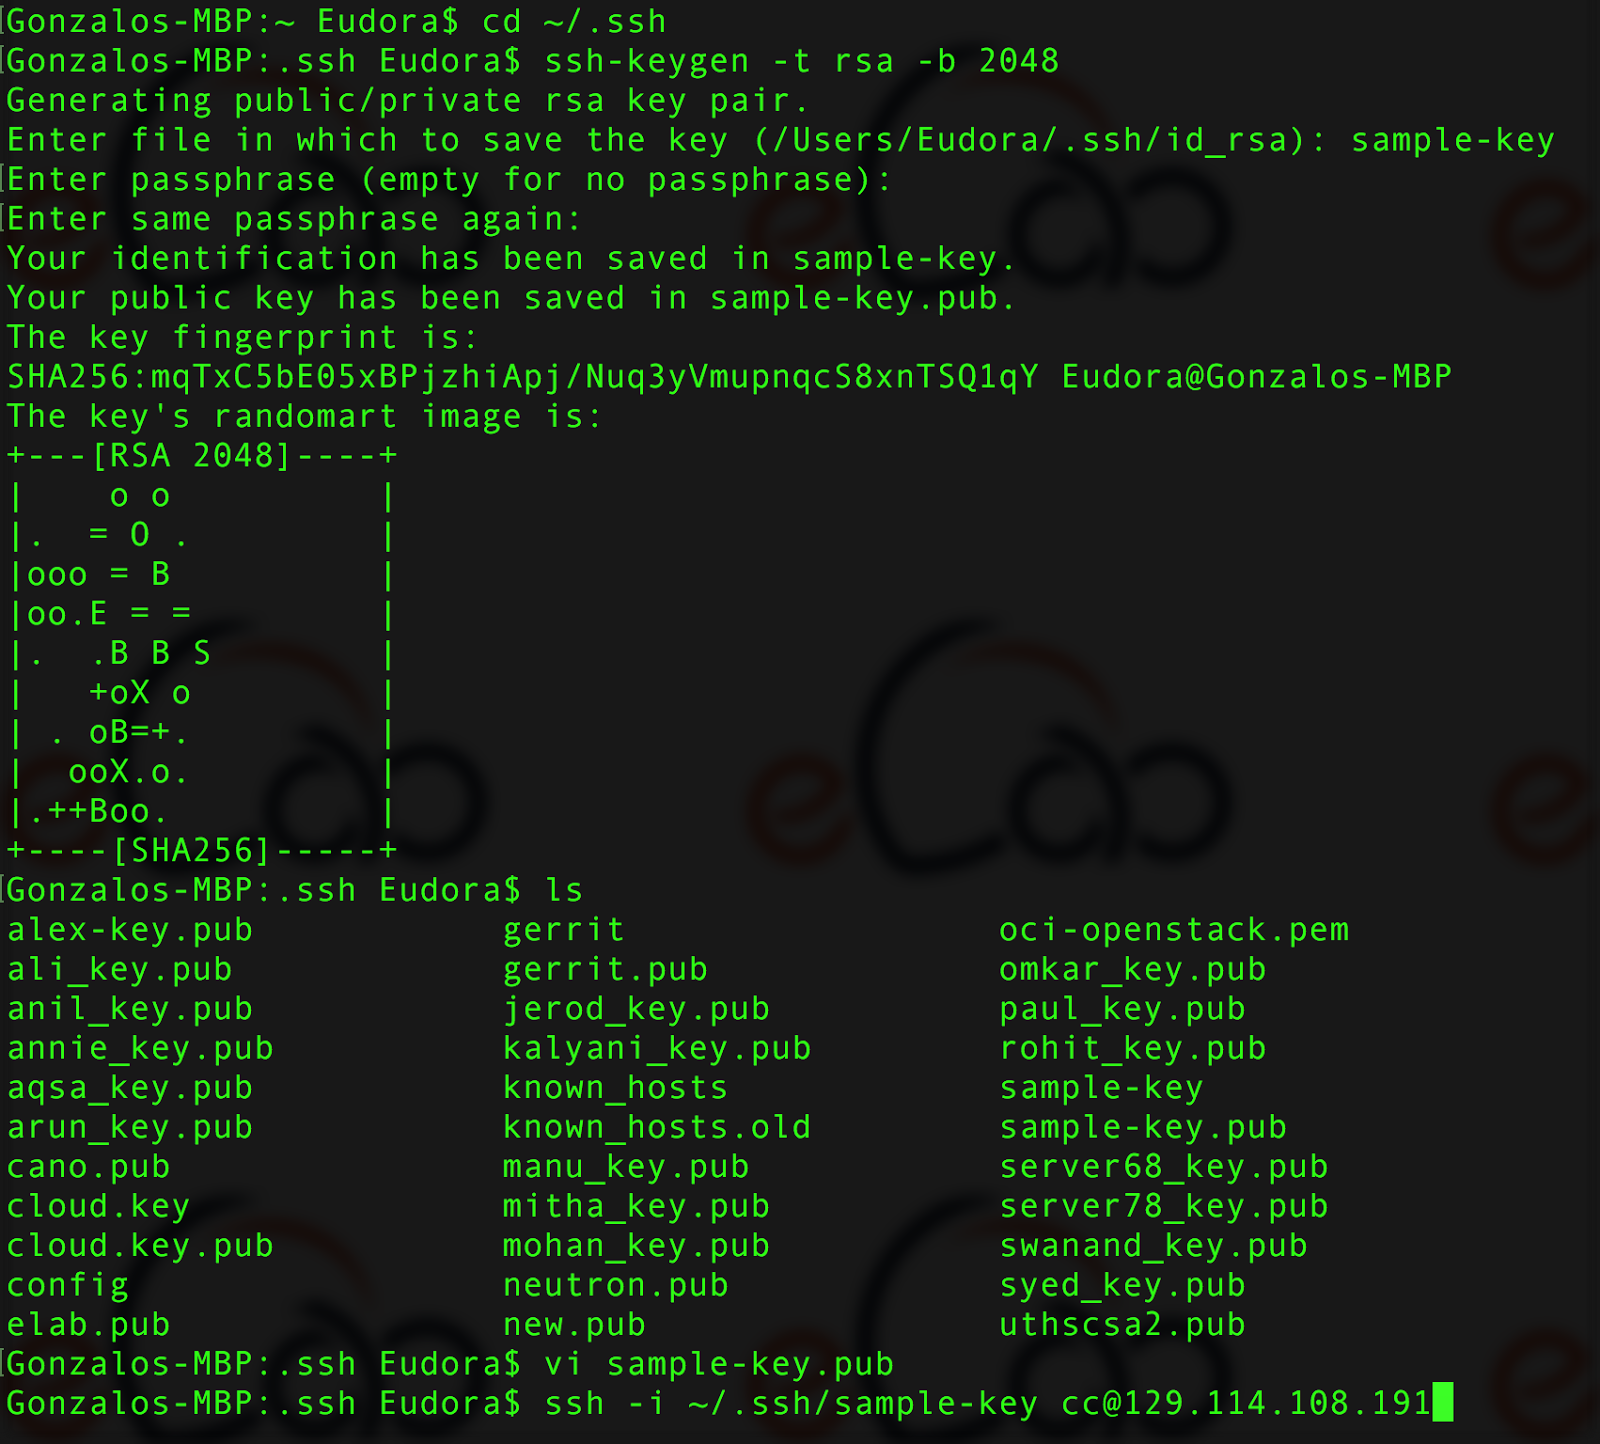
\includegraphics[width=\columnwidth]{images/chameleon/ssh1.png}}

\subsection{For Windows}\label{for-windows}

First, download and install PuTTY and PuTTYgen
\href{http://www.chiark.greenend.org.uk/~sgtatham/putty/}{from here}.
Once downloaded, opening PuTTYgen will open a key generator window, seen
below.

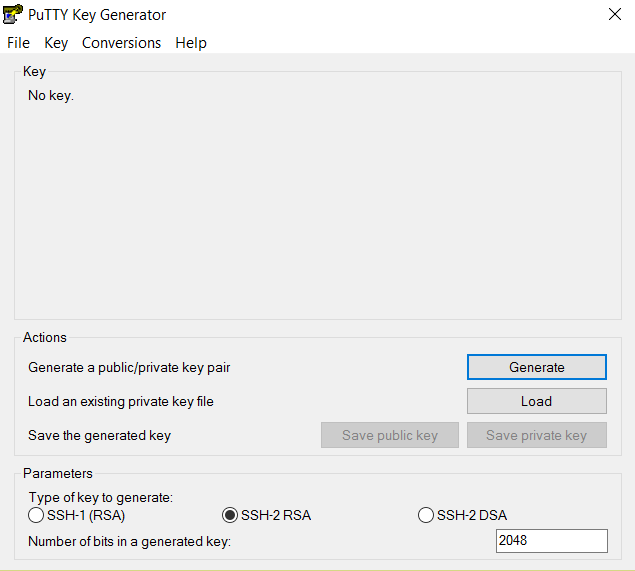
\includegraphics[width=\columnwidth]{images/chameleon/putty2.png}

Once the program is opened, click the Generate button, seen above in
blue.~PuTTY Key Generator will then ask you to move your mouse around
the program's blank space to generate ``randomness'' for your key.?

You may enter an optional~``Key passphrase'' and then confirm the
passphrase in the required areas but let us keep these~spaces in blank
just to avoid complexity. An example is shown below. Note that the
passphrases are not necessary!

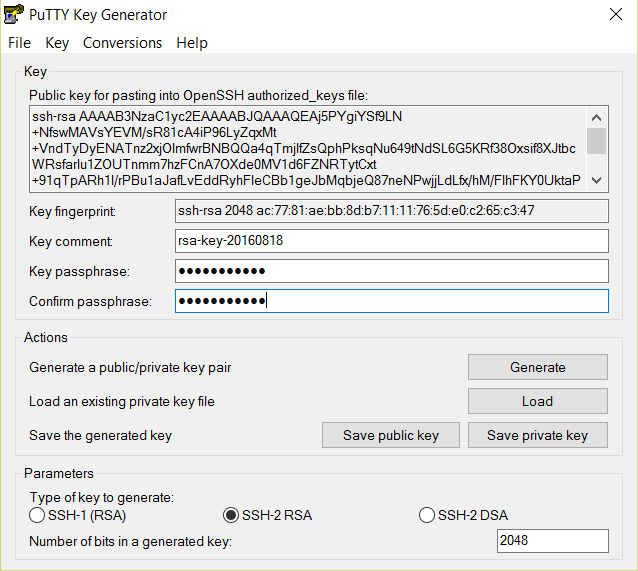
\includegraphics[width=\columnwidth]{images/chameleon/putty3.png}

Save both the public and private keys into a file of your choice using
the ``Save public key'' and ``Save private key'' buttons; name them
something obvious like ``public\_key'' and ``private\_key'' so that you
can distinguish between the two.

Before closing this window, select the entire public key and copy it
with ``Control-C''. Please note that everything should be copied,
including ``ssh-rsa''. This will be used when importing the key pair to
Openstack.

At this time, the public key has been created and copied. Now you can
now follow the steps described above (starting with the line ``Provide
the public key to your cloud system or individual instance'') to import
the generated key pair for use with Chameleon!
